\chapter{Анализ структуры локальных оптимумов} \label{sec:exp}
Процедура решения задачи оптимизации ФАР при ограничении мощности по каждой точке питания состоит в следующем:
%
\begin{enumerate}
  \item Для каждого излучателя в решетке рассчитать парциальные компоненты полей $f_i^{(l)}, i= \overline{1,N}, l=\overline{1,2}$.
  \item Вычислить матрицы $\textbf{G}$ and $\textbf{H}^{(k)},\ k=\overline{1,n},$ из подраздела~\ref{subsec:statement}.
  \item Оценить радиус допустимой области используя формулы из подраздела~\ref{subsec:top}.
  \item Решить задачу~(\ref{eq:task3}) с дополнительными ограничениями $x_N = 0, ||\textbf{x}||\le \sqrt{\frac{N}{\lambda_{\min}}}$.
\end{enumerate}

Данный подход может гарантировать нахождение как локального, так и глобального оптимума, в зависимости от решателя, используемого на шаге~4. Как один из базовых оптимизационных методов, мы рассматриваем метод градиентной оптимизации (максимизационный вариант)
с алгоритмом одномерного поиска Дэвиса, Свенна и Кэмпи~(ДСК)~\cite{himmelblau:nlp}. Далее целевая функция задачи~(\ref{eq:task3}) будет обозначатся символом $\tilde{F}$.

В нашей работе от задачи условной оптимизации мы переходим к задаче безусловной оптимизации методом штрафных функций, а именно -
методом внешней точки~\cite{eremin:convex,aoki:mo}:
\begin{equation}
       \textbf{x}^{T}\textbf{Gx} - r\cdot \sum_{k=1}^n
       \left( \min\left(0,\textbf{x}^{T}\textbf{H}^{(k)}\textbf{x}\right) +
       \min\left(0,1-\textbf{x}^{T}\textbf{H}^{(k)}\textbf{x}\right)\right)^4 \rightarrow
       \max,
     \label{eq:task4}
\end{equation}
где $r$ - достаточно большой штрафной параметр. Глобально-оптимальное решение для задачи~(\ref{eq:task4}) может не быть допустимым для изначальной задачи~(\ref{eq:task3}), но увеличение штрафного параметра~$r$ уменьшает нарушение ограничений. Кроме того, имея решение~$\textbf{x}$, которое нарушает в задаче~(\ref{eq:task3}) только неравенства вида $\textbf{x}^{T}\textbf{H}^{(k)}\textbf{x} \leq 1$, мы будем ссылаться на результаты градиентной оптимизации с использованием восстановления допустимости~(\ref{eq:scale}) после срабатывания критерия остановки. Алгоритм градиентной оптимизации повторяется многократно, при этом используется случайно сгенерированный вектор~$\textbf{x}\in \mathbb{R}^{2N}$ в качестве стартовой точки. Распределение случайной величины $\textbf{x}$ описано в подразделе~\ref{subsec:results}. Для каждого найденного решения выполняется проверка на удовлетворение необходимым условиям локальной оптимальности путем решения задачи~(\ref{eq:task5}). Затем, решение линеаризованной задачи, удовлетворяющее  необходимым условиям локальной оптимальности, снова подается на вход алгоритма градиентной оптимизации, остальные решения отсеиваются. Последний шаг применяется, поскольку решение задачи~(\ref{eq:task5}) может оказаться за пределами допустимой области задачи~(\ref{eq:task3}). В этом случае данный этап показывает, как далеко решение линеаризованной задачи находится от решения, найденного градиентным алгоритмом.

С целью отыскания глобального оптимума задачи~(\ref{eq:task3}) посредством решателя BARON~\cite{tawarmalani:global}, основанного на методе ветвей и границ с использованием локальной оптимизации для поиска начального приближения, необходимо предоставить ограничивающий параллелепипед или верхнюю оценку евклидовой нормы допустимых решений. Для этого может быть использовано неравенство~(\ref{eqn:bound}). Для всех решаемых в этом эксперименте задач была рассмотрена возможность применения процедуры сужения допустимой области.

\section{Тестовые примеры}\label{subsec:examples}

Вычислительный эксперимент был поставлен для задач, построенных на основе четырех типов ФАР: широкополосных вертикальных излучателей, широкополосных вертикальных диполей и симметричных вертикальных диполей. При моделировании полей был использован пакет NEC2, для которого были предоставлены соответствующие геометрические конфигурации антенных систем. В качестве рабочей частоты было выбрано 5МГц. Рассмотрены квадратные ФАР конфигурации 2x2, 3x3 и 5x5. Заранее отметим, что конфигурация 5x5 была рассмотрена только для решеток СВД, поскольку NEC2 не смог обработать 5x5~ШВИ и 5x5~ШВД из-за высокой сложности этих моделей. В случае с ФАР кольцевой структуры были рассмотрены решетки, состоящие из 8 и 16 излучателей.

Решетки ШВИ смоделированы расположенными на высоте 0.2 метра над поверхностью земли (проводимость земли равна~0.01~См/м, относительная диэлектрическая проницаемость~10). Решетки ШВИ и СВД размещены в свободном пространстве. В случае ШВЕ и ШВД, расстояние между соседними излучателями равно 20~метров. Высота каждого излучателя ШВИ равна 15~метров. Расстояния между концами каждого излучателя ШВД равно 30 метров. В случае СВД, были рассмотрены два типа излучателя: с длинами излучателя~10~и~30~метров и расстояниями между соседними излучателями 5 и 10 метров соответственно. СВД с длиной излучателя равной 10~метрам в исследовании помечены штрихом (СВД'). Система противовесов ФАР кольцевой структуры поднята над землей на 2 м. для того, чтобы ослабить влияние потерь в земле. Расстояние между соседними излучателями в этих ФАР равно 8 м. В качестве направления максимизации излучения выбраны: азимутальный угол $45^{\circ}$, полярный угол $70^{\circ}$.

\section{Результаты вычислительного эксперимента} \label{subsec:results}

В этом разделе мы сравниваем результаты работы градиентного метода и решателя BARON в его режиме по умолчанию. Во всех экспериментах, описанных ниже, было установлено ограничение по времени 1000с. Все эксперименты проводились на ЭВМ с процессором Intel i7 (тактовая частота: 2.8ГГц), ОЗУ: 16Гб. В случае сходимости градиентного метода (завершение по минимально допустимому приращению целевой функции $10^{-4}$), алгоритм перезапускается заново до истечения запаса времени.

Для каждой задачи была применена процедура получения верхней оценки нормы допустимых решений~(c.м. подраздел \ref{subsec:top}). При выполнении этой процедуры для многих задач получались близкие к нулю (или даже нулевые) собственные числа, что делало невозможным их дальнейшее использование для оценки нормы $\sqrt{\frac{N}{\lambda_{\min}}}$. В таблице~\ref{tab:results} такие оценки задачи отмечены прочерком в соответствующем столбце. Так как из физических соображений собственные числа должны быть строго больше 0, проблемы с вычислением верхней оценки нормы допустимых решений свидетельствуют о допущенной погрешности при вычислении матриц, определяющих квадратичные формы задачи~(\ref{eq:task3}). В частности, одной из таких проблем является несимметричный вид вещественных матриц. В таком случае, их следует привести к симметричному ввиду путем усреднения симметричных относительно главной диагонали компонент.

Во время каждой инициализации градиентного метода стартовая точка~$\textbf{x}$ выбирается независимо с равномерным распределением в кубе $[-5000, 5000]^{2N}$. Такой выбор оказался достаточным для всех задач, кроме СВД~2x2, чтобы получить решение, по целевой функции соответствующее решению, предоставляемому решателем BARON. Лучшее из найденных таким образом решений принимается за конечный результат. Параметр штрафа~$r$ в методе градиентной оптимизации установлен равным $10^6$ на всех запусках. Такое значение было определено эмпирически. В таблице~\ref{tab:results} приводятся результаты вычислительного эксперимента. Значения целевой функции ``$\tilde{F}$'' точке, полученной алгоритмом градиентного подъема, приводятся после процедуры масштабирования~(\ref{eq:scale}). Для решателя BARON версии~18.5.8 было выбрано то же самое ограничение сверху на процессорное время, что и для градиентного метода (группа колонок ``BARON''), и 50000с. для проверки глобальной оптимальности. Во всех таблицах, колонка ``t'' содержит время до получения лучшего найденного решения или до установления глобальной оптимальности. Во всех запусках градиентного метода были получены решения, где активными оказались все ограничения вида $\textbf{x}^{T}\textbf{H}^{(k)}\textbf{x} \leq 1$.

\begin{table}[!h]
\centering
\begin{tabular}{|c|c|c|c c|c c|}
    \hline
    \multirow{2}{*}{\textbf{Тип}} & \multirow{2}{*}{$\lambda_{min}$} & \multirow{2}{*}{$\sqrt{\frac{N}{\lambda_{\min}}}$} & \multicolumn{2}{c}{\textbf{Град.}} & \multicolumn{2}{|c|}{\textbf{BARON}}\\
    & & & \textbf{$\tilde{F}$} & \textbf{t, c} & \textbf{$\tilde{F}$} & \textbf{t, c} \\
    \hline
    ШВИ 2х2 & 0.0215 & 13.6 & 138.2 & \textbf{0.054} & \textbf{139.2} & 0.12 \\
    ШВИ 3х3 & 0.0177 & 70 & 575.7 & 0.93 & \textbf{580.6} & \textbf{0.34} \\
    ШВД 2х2 & 0.009 & 21 & 459.7 & \textbf{0.13} & \textbf{463.6} & 0.27 \\
    ШВД 3х3 & 0.0013 & 6767 & 915 & 24.4 & \textbf{925} & \textbf{0.34}  \\
    СВД 2х2 & $2\cdot10^{-3}$ & 44& 357 & 1.9 & \textbf{361} & \textbf{0.16} \\
    СВД 3х3 & $5.6\cdot10^{-9}$ & $8.4\cdot10^{5}$& 1138 & 25.6 & \textbf{1261} & \textbf{0.38}\\
    СВД 5х5 & - & - & 5318 & 1000 & \textbf{6716} & 1000 \\
    СВД' 2х2 & $7.76\cdot10^{-9}$ & $22\cdot10^{3}$ & 233 & 2.52 & \textbf{253} & \textbf{0.25} \\
    СВД' 3х3 & 0.0008 & $1\cdot10^4$& 664 & 71 & \textbf{1153} & \textbf{1.48} \\
    СВД' 5х5 & - & - & \textbf{1382.7} & 1000 & 33.5 & \textbf{217.94}  \\
    Кольц. 8 & $3\cdot10^{-3}$ & 154 & 217 & 8.06 & \textbf{218} & \textbf{0.23} \\
    Кольц. 16 & $6.7\cdot10^{-4}$ & $1.2\cdot10^{6}$& 727 & 90.9 & \textbf{734} & \textbf{1.37} \\
    \hline
\end{tabular}
\caption{ Результаты оптимизации, полученные с помощью градиентного подъема и решателя BARON.}
\label{tab:results}
\end{table}

Из таблицы~\ref{tab:results} видно, что на всех видах решеток, кроме решеток СВД конфигураций~3x3 и~5x5, а также СВД' конфигураций~2x2 и~3x3, разница в значениях целевой функции не превосходит 1\%. Для решеток СВД конфигураций~3x3 и~5x5, а также СВД' конфигураций~2x2 и~3x3 градиентный алгоритм существенно уступает по качеству найденного решения. Более детальное исследование для СВД' конфигураций 2x2 и 3x3 показало, что BARON предоставляет решение с очень малой областью притяжения. Суть такого исследования заключалась в том, что к решению, полученному с помощью решателя BARON добавлялось некоторое возмущение, после чего модифицированная точка подавалась на вход градиентного алгоритма. Очень малые возмущения (до 0.5\% относительно нормы решения) исходной точки не мешали градиентному алгоритму найти точку, лежащую в окрестности решения, найденного с помощью решателя BARON. Однако, принимая на вход возмущенное порядка 0.5\% относительно нормы решение решателя BARON, градиентный подъем приводил к решению со значением целевой функции $\tilde{F} = 233$  в случае СВД'~2x2. При этом, используемая нами процедура проверки локальной оптимальности не дала опровержения локальной оптимальности решения со значением целевой функции $\tilde{F} = 253$, предоставленного решателем BARON. Аналогичные результаты были получены как для СВД, так и для СВД' конфигурации~3x3. Особое внимание привлекают решетки СВД и СВД' конфигурации 5x5, поскольку за предоставленный временной промежуток градиентный подъем так и не достиг критерия остановки. BARON в случае СВД'~5x5 за это же время достиг решения, значительно хуже по целевой функции. Вероятно, как BARON, так и градиентный подъем сошлись бы к более качественному решению, если бы не были ограничены по времени. Кроме решeток ШВИ и ШВД конфигурации~2x2 BARON демонстрирует лучшее время счета. Однако, следует отметить, что для обоих алгоритмов время, затраченное на поиск решения, было либо существенно меньше, либо сравнимо со временем, затраченным на построение исходных данных пакетом моделирования NEC, что делает оба подхода равноценными по времени работы с практической точки зрения. Важным результатом, не приведенным в таблице~\ref{tab:results}, является то, что для ФАР конфигураций ШВИ~2x2, ШВД~2x2 и ШВИ~3x3 была доказана глобальная оптимальность найденного решателем BARON решения.

В качестве иллюстрации физических свойств полученных решений, на рис.~\ref{ris:bve_comp} приведен горизонтальный план диаграммы направленности ФАР для решений, найденных с помощью метода градиентной оптимизации. Под диаграммой направленности понимается графическое представление зависимости коэффициента усиления антенны от ее направления в заданной плоскости. Такая диаграмма позволяет наглядно оценить, на какое направление приходится максимум излучения, и провести качественную оценку работы алгоритма. На рис.~\ref{ris:bve_comp} изображена диаграмма направленности для решетки ШВИ размера 2x2 (пунктирная линия) и ШВИ 3x3 (сплошная линия). Для решений, полученных с помощью решателя BARON для этих задач, диаграммы аналогичны. Еще раз отметим, что при эксперименте направление оптимизации было представлено углами в полярных координатах: азимутальный угол был принят равным $45^{\circ}$, полярный угол - $70^{\circ}$. Как видно из горизонтального плана диаграммы направленности при значении полярного угла $70^{\circ}$, максимальному излучению соответствует направление оптимизации $45^{\circ}$. Сравнение диаграмм показывает, что использование решеток с большим числом излучателей позволяет уменьшить излучение в других направлениях.

\begin{figure}[h]
    \centering
    \center{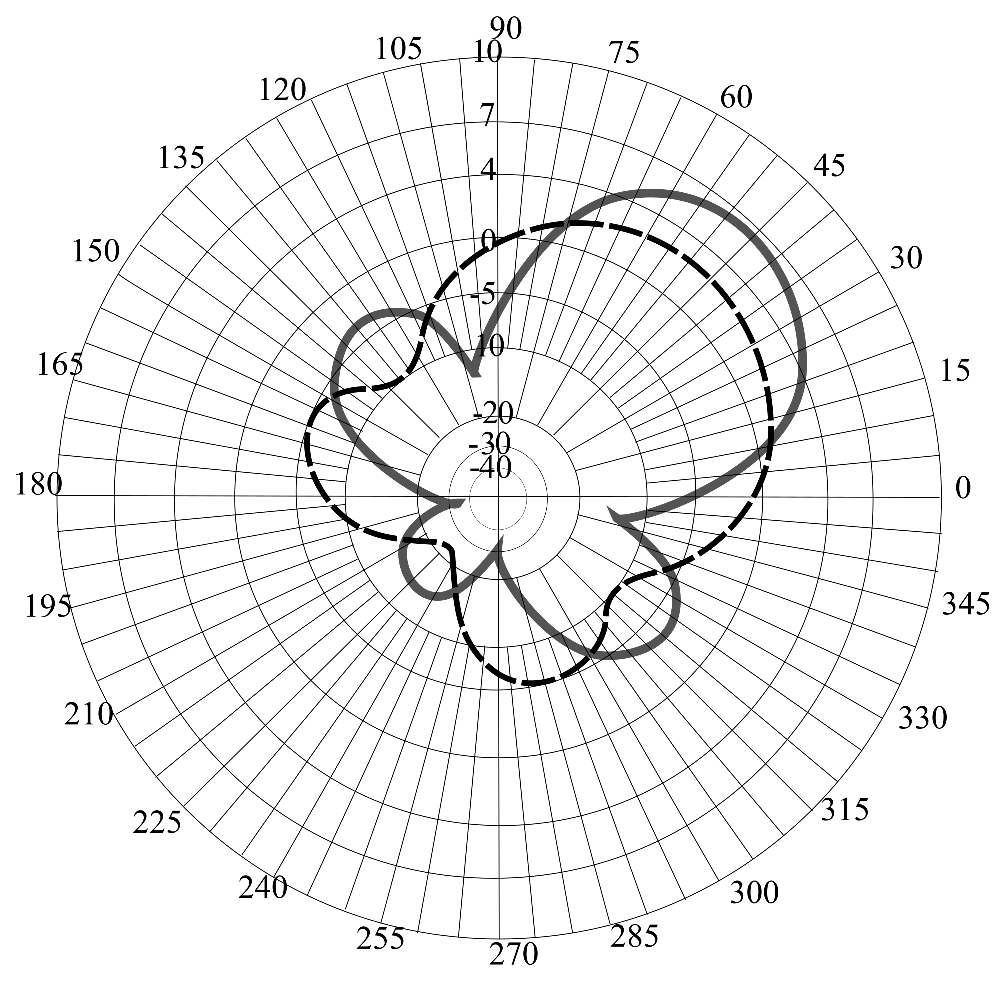
\includegraphics[width=0.5\linewidth]{BWE_comp.eps} }
    \vspace{0.7em}
    \caption{Горизонтальный план диаграммы направленности для решетки ШВИ 2x2 (пунктир) и ШВИ 3x3 (сплошная)}
    \label{ris:bve_comp}
\end{figure}

\section{Количество локальных оптимумов и их расположение}\label{subsec:analyzeloc}
\begin{table}[!h]
\centering
\begin{tabular}{|l | l l | c c c | c c c|}
    \hline
    \textbf{ФАР} & \textbf{$M$} & \textbf{$M_{ne}$} & \textbf{$M_{f}$} & \textbf{$\mathcal{B}_{M_f}$} & \textbf{$\mathcal{L}_{M_f}$} & \textbf{$M_{y\approx0}$} & \textbf{$\mathcal{B}_{M_{y\approx0}}$} & \textbf{$\mathcal{L}_{M_{y\approx0}}$}\\
    \hline
    ШВИ 2x2 & 18368 & 4 & 1 & 1 & 1 & 4 & 4 & 4\\
    ШВД 2x2 & 7678  & 4 & 1 & 1 & 1 & 4 & 4 & 4\\
    СВД 2x2  & 523  & 1 & 1 & 1 & 1 & 1 & 1 & 1\\
    СВД 3x3  & 39  & 9 & 2 & 2 & 2 & 5 & 5 & 5\\
    СВД' 2x2  & 396  & 370 & 3 & 3 & 3 & 338 & 1000 & 1213\\
    СВД' 3x3  & 14  & 14 & 3 & 3 & 3 & 1 & 1 & 1\\
    ШВИ 3x3 & 1070  & 3 & 1 & 1 & 1 & 3 & 3 & 3 \\
    ШВД 3x3 & 41  & 4 & 4 & 4 & 4 & 1 & 1 & 1 \\
    Кольц. 8 & 124  & 9 & 2 & 2 & 2 & 9 & 9 & 9\\
    Кольц. 16 & 11  & 6 & 1 & 1 & 1& 6 & 6 & 6\\
    \hline
\end{tabular}
    \caption{Структура локальных оптимумов.}
    \label{tab:structure}
\end{table}

\begin{figure}
\centering
    \begin{minipage}[h]{0.8\linewidth}
            \center{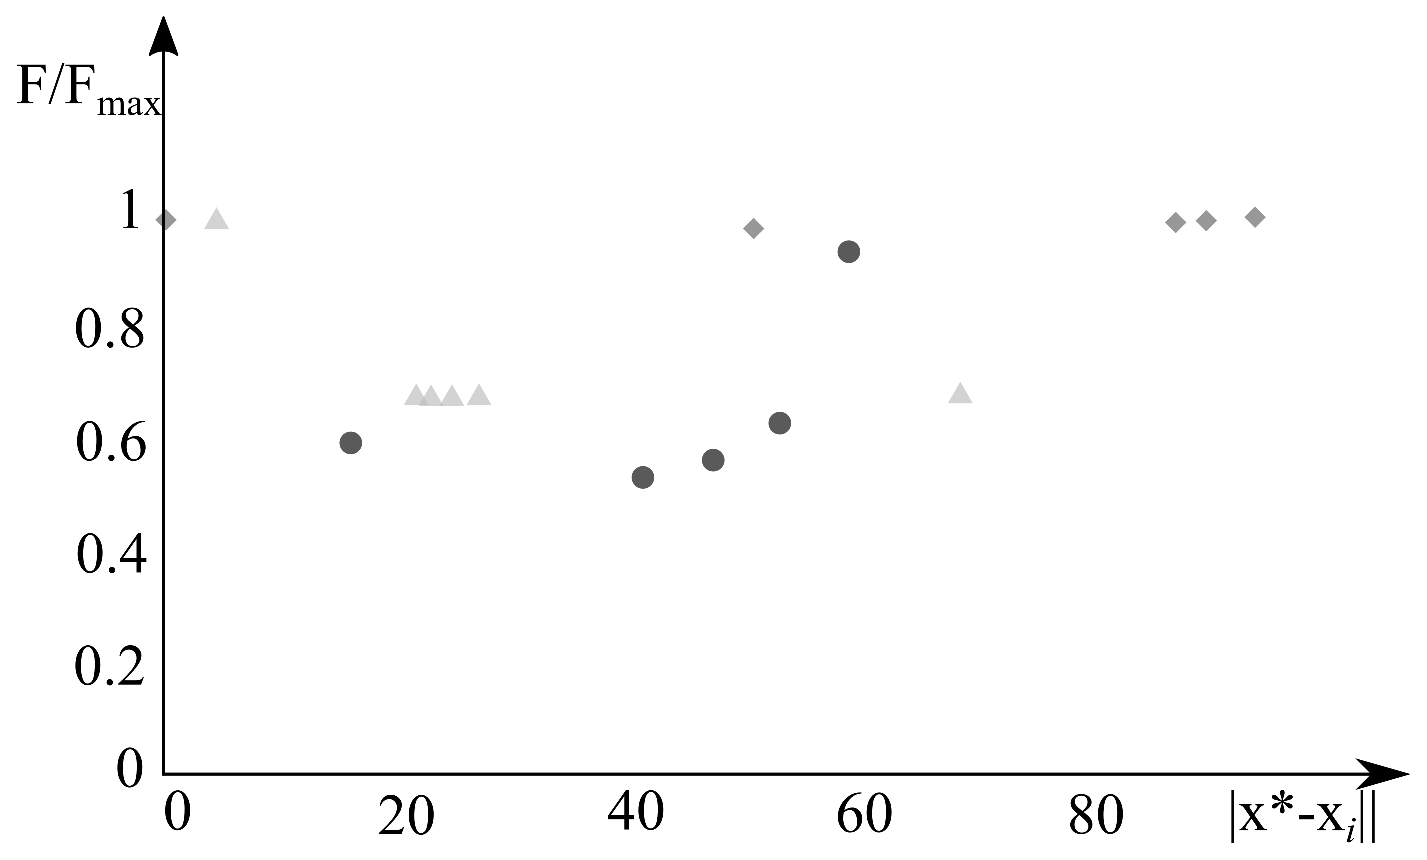
\includegraphics[width=0.9\linewidth]{fit_dist.eps}  \\ а) }
    \end{minipage}
    \begin{minipage}[h]{0.8\linewidth}
            \center{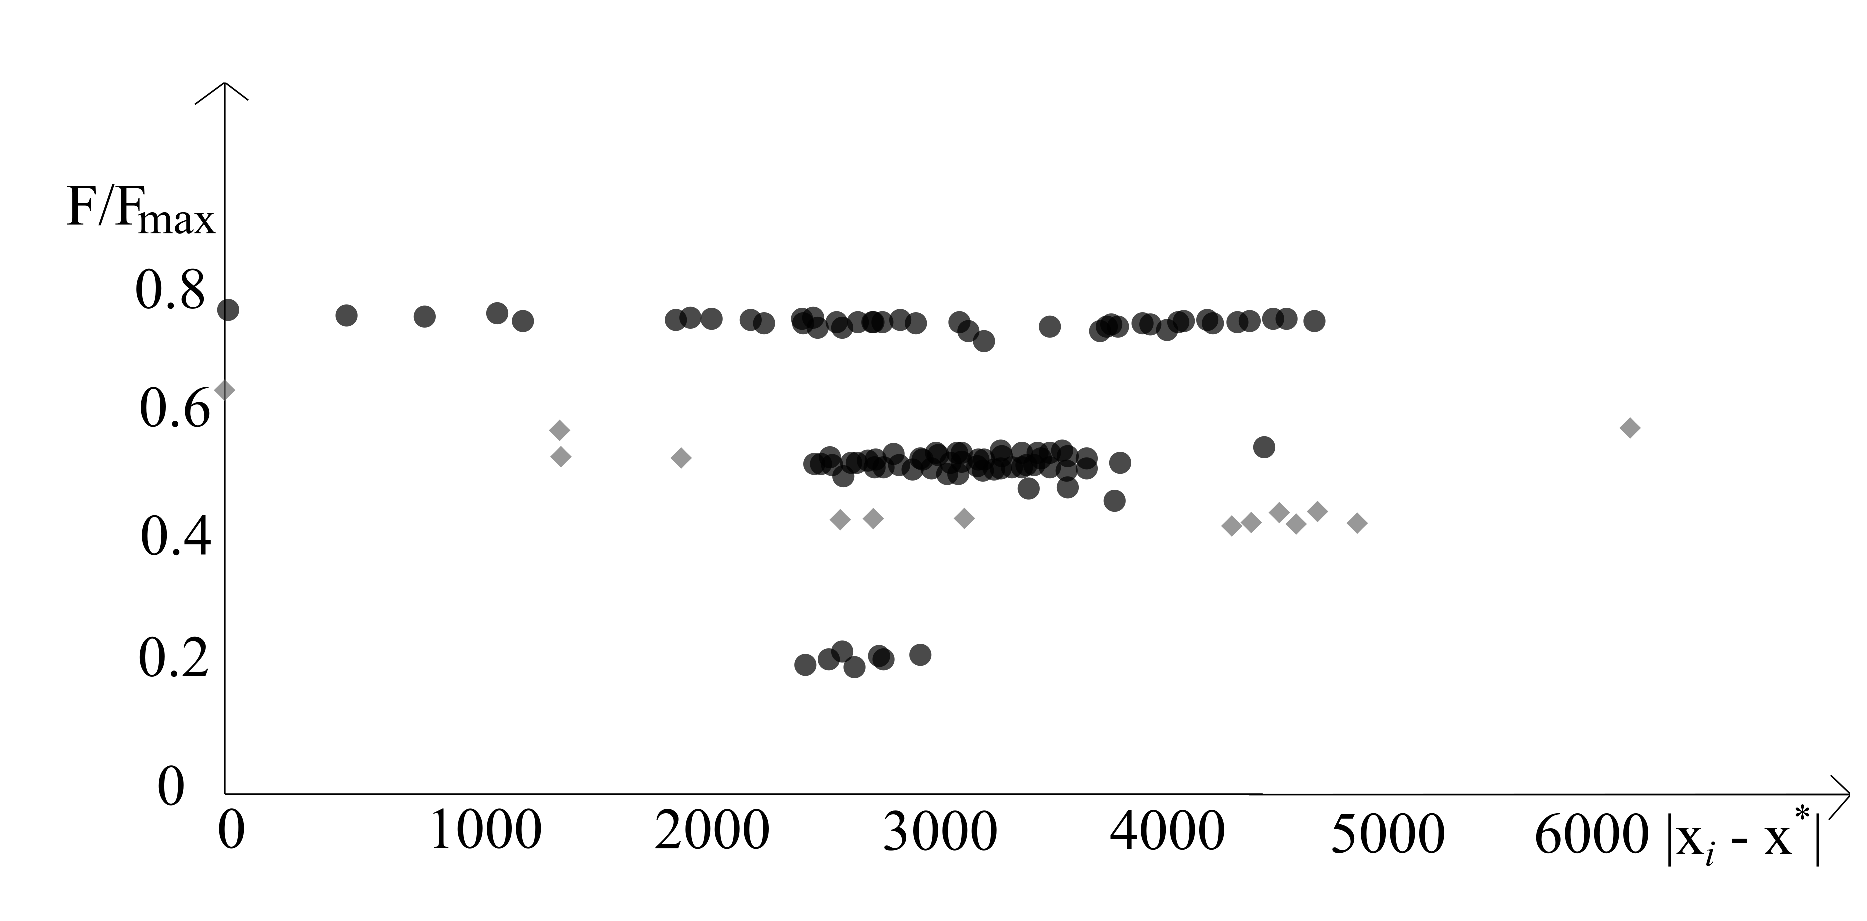
\includegraphics[width=0.9\linewidth]{fit_dist_2x2.eps}  \\ б) }
    \end{minipage}
    \vspace{0.7em}
    \caption{Структура множества найденных решений для задач ШВИ, ШВД, СВД (а) и СВД' (б)}
    \label{ris:fit_dist}
\end{figure}

Для оценки общего числа локальных оптимумов использовался метод переписи Шнабеля. Данный метод имеет применение в экологии и заключается в
выводе статистических оценок численности популяции на основе числа особей, помеченных в результате эксперимента, из популяции с неизменным
составом, где каждая особь имеет константную вероятность отлова. В~\cite{eremeev:confidence} предлагается адаптация такого метода для оценки числа локальных оптимумов. В таблице~\ref{tab:structure} приводится статистика по числу различных точек остановки (в пределах заданной точности) процедуры мультистарта в течение 1000~с. процессорного времени. Для каждого решения была применена процедура линеаризации задачи и проверки необходимых условий локальной оптимальности, описанная в разделе~(\ref{sec:loc}). Приемлемыми считались отличия целевой функции линеаризованной задачи от значения целевой функции, найденного градиентным методом менее чем на 1\%. Здесь {$M$} - число выполненных запусков за отведенное время, $M_{ne}$ - число групп решений, отличающихся не более чем на 10\% по каждой из координат, {$M_{f}$} - число групп значений целевой функции у таких неэквивалентных решений (с точностью до 10\%, приведенных в таблице~\ref{tab:results}). {$M_{y\approx0}$} - число групп решений, для которых были выполнены необходимые условия локальной оптимальности. $\mathcal{B}$ и $\mathcal{L}$ - оценка нижней границы и оценка максимального правдоподобия числа локальных оптимумов, рассчитанные по методу переписи Шнабеля. Доверительная вероятность для данного метода была выбрана равной 95\%. Оценки для числа решений с различными значениями целевой функции обозначены $\mathcal{B}_{M_f}$ и $\mathcal{L}_{M_f}$. Оценки для числа решений, для которых были выполнены необходимые условия локальной оптимальности, обозначены $\mathcal{B}_{M_{y\approx0}}$ и $\mathcal{L}_{M_{y\approx0}}$.
В случае СВД и СВД' конфигурации 5x5 в течение 1000~с градиентный метод не достиг решения, удовлетворяющего условию остановки, поэтому
данный результат не включен в таблицу~\ref{tab:structure}.

Как видно из таблицы, во всех экспериментах в некоторых запусках были найдены неразличимые с практической точки зрения решения. Для квадратных решеток ШВИ и ШВД было найдено по одному такому решению. Решетки кольцевой структуры и СВД'~2x2 имеют значительное разнообразие как по найденным векторам решений, так и по значениям целевой функции. Относительно решений, для которых были выполнены необходимые условия локальной оптимальности, можно сказать, что с большой вероятностью для задачи СВД'~2x2, были найдены далеко не все возможные решения. О решетке СВД'~3x3 известно, что градиентный подъем был остановлен в точке, не лежащей в окрестности решения, предоставляемого решателем BARON.

На рис.~\ref{ris:fit_dist} приведены диаграммы локальных оптимумов, где по оси ординат отложены значения целевой функции, а по оси
абсцисс - расстояние до лучшего известного решения. В случае а) точками обозначены результаты для кольцевых решеток, состоящих из 8 излучателей, ромбами - для кольцевых решеток, состоящих из 16 излучателей, пятиугольниками - для СВД~3x3. В случае б) точками обозначены результаты для СВД'~2x2, ромбами - для СВД'~3x3. Диаграмма показывает, что значения, соответствующие одному и тому же значению целевой функции, могут находиться достаточно далеко друг от друга, что позволяет сделать предположение о наличии неучтенных симметрий задачи (о множестве линейных симметрий задачи см. в~\cite{yurkov:symmetry}).

\section{Экспериментальная проверка устойчивости решений}
\begin{figure}[h]
    \centering
    \center{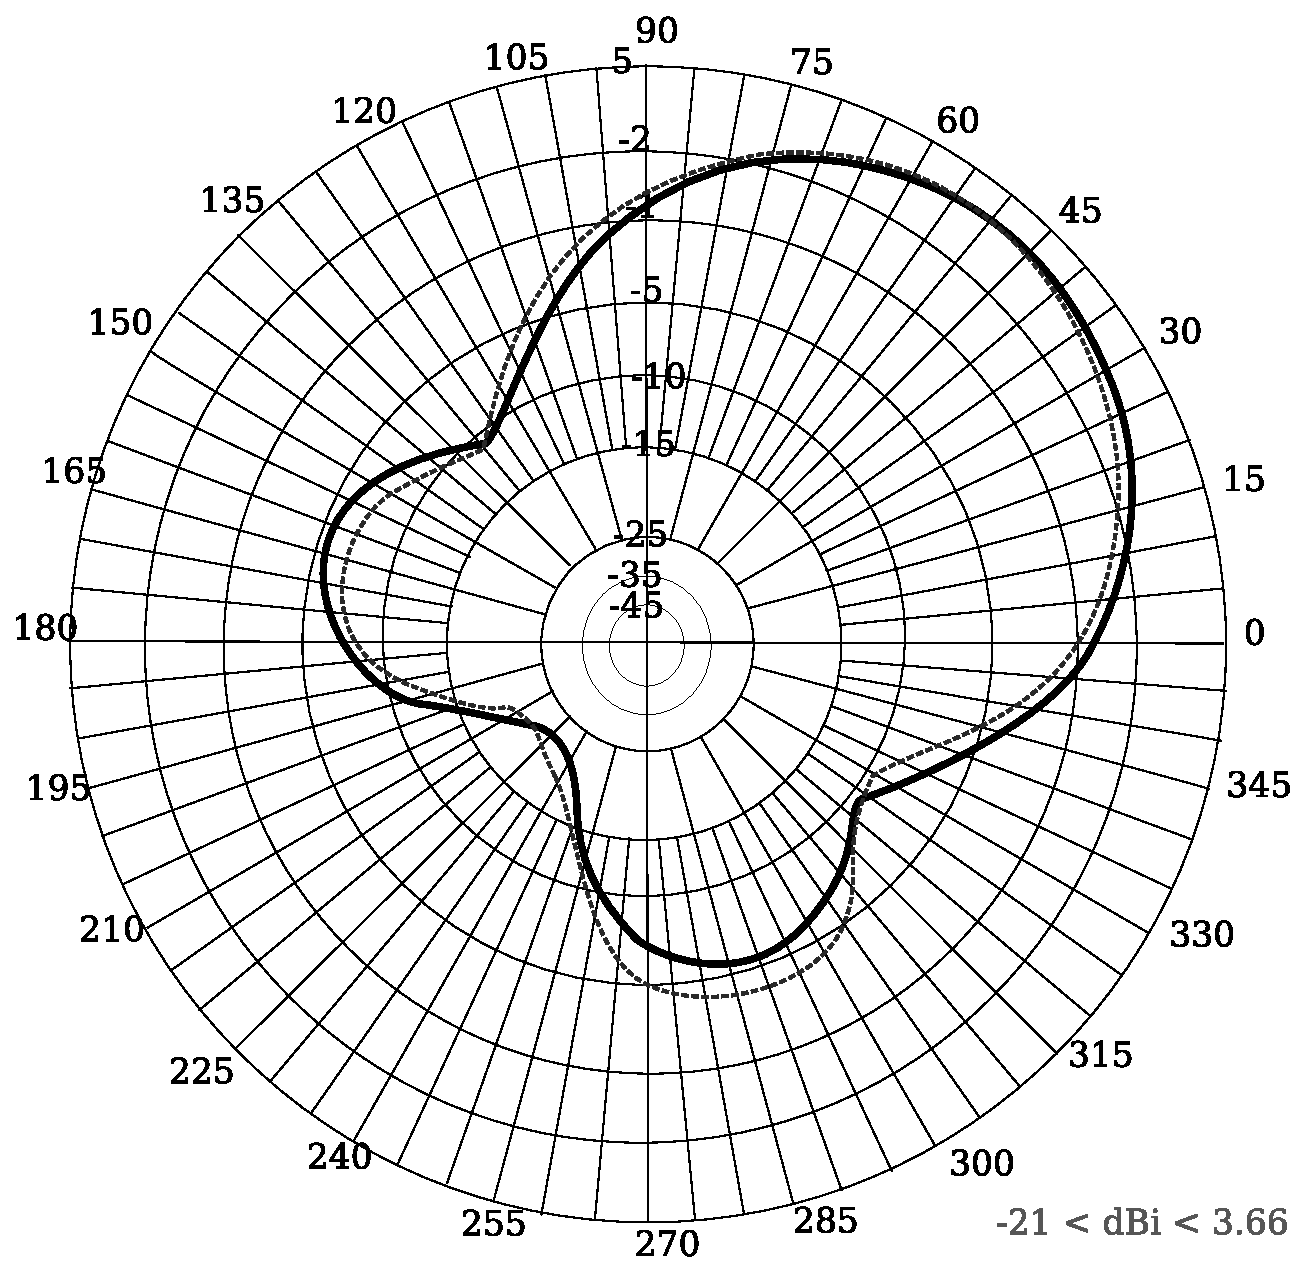
\includegraphics[width=0.5\linewidth]{stability.eps} }
    \vspace{0.7em}
    \caption{Диаграммы направленности для ШВИ~2x2 при оптимизации в направлении 70:45 (сплошная линия) и 70:50 (пунктир)}
    \label{ris:bve_comp}
\end{figure}
При анализе структуры локальных оптимумов может возникнуть вопрос об устойчивости решения по аргументу. В данной работе было проведено исследование изменения значения целевой функции при изменении оптимизируемого направления на малый угол. В рассмотрение принималось также изменение значения целевой функции при подстановки в исходную задачу решения, найденного для нового направления (для удобства вывода результата такая подстановка обозначена за P1), и наоборот - при подстановке в задачу для измененного направления решения, полученного для исходного направления (обозначается P2). Исследование проводилось на квадратных решетках, состоящих из 4-х и 9-и излучателей. Азимутальный и полярный угол менялись на $5^{\circ}$. Результаты приведены в таблице~\ref{tab:stability}
\begin{table}[!h]
\centering
\begin{tabular}{|c|c|c|c|c|c|c|c|}
    \hline
    \textbf{ФАР} & \textbf{Подстановка} & \textbf{70:45} & \textbf{75:45} & \textbf{65:45} & \textbf{70:50} & \textbf{75:40} & \textbf{65:50}\\
    \hline
    \multirow{3}{*}{ШВИ 2x2} & - & \multirow{3}{*}{138} & 125 & 138 & 137 & 137 & 125\\
    & P1 &  & 138 & 138 & 137 & 137 & 137\\
    & P2 &  & 125 & 138 & 136 & 136 & 123\\
    \hline
    \multirow{3}{*}{ШВИ 3x3} & - & \multirow{3}{*}{575} & 532 & 565 & 574 & 533 & 564\\
    & P1 &  & 574 & 572 & 560 & 558 & 557\\
    & P2 &  & 530 & 562 & 559 & 517 & 546\\
    \hline
    \multirow{3}{*}{ШВД 2x2} & - & \multirow{3}{*}{459} & 518 & 454 & 454 & 512 & 389\\
    & P1 &  & 458 & 459 & 457 & 456 & 389\\
    & P2 &  & 518 & 392 & 452 & 510 & 386\\
    \hline
    \multirow{3}{*}{ШВД 3x3} & - & \multirow{3}{*}{1501} & 1817 & 872 & 1015 & 1196 & 1198\\
    & P1 &  & 1506 & 1047 & 1000 & 1004 & 1448\\
    & P2 &  & 1774 & 1203 & 1450 & 1713 & 1162\\
    \hline
    \multirow{3}{*}{СВД 2x2} & - & \multirow{3}{*}{369} & 417 & 315 & 365 & 412 & 312\\
    & P1 &  & 368 & 369 & 367 & 366 & 367\\
    & P2 &  & 417 & 315 & 363 & 410 & 310\\
    \hline
    \multirow{3}{*}{СВД 3x3} & - & \multirow{3}{*}{1484} & 1789 & 1176 & 1459 & 1162 & 1753\\
    & P1 &  & 1475 & 1472 & 1446 & 1428 & 1444\\
    & P2 &  & 1782 & 1164 & 1427 & 1120 & 1713\\
    \hline
\end{tabular}
    \caption{Значения целевой функции при изменении оптимизируемого направления на малый угол.}
    \label{tab:stability}
\end{table}

Результаты исследования показывают, что изменение направления оптимизации на малый угол соответствуют повороту исходной диаграммы направленности на этот угол.

\section{Исследование непрерывных симметрий}

Solution and analysis of mathematical programming problems may be simplified when these problems are symmetric under appropriate linear transformations. In particular, a knowledge of the symmetries may help reduce the problem
dimension, cut the search space by symmetry-breaking linear cuts or obtain new
local optima from the ones previously found. These methods are applicable in
the case of a continuous solutions domain [3, 6, 8] as well as in the integer programming [1, 2, 7, 11, 16] and in the mixed integer programming [10, 12]. While
most of the applications of symmetries are aimed at speeding up the exact optimization algorithms, yet in some cases the knowledge of symmetries may also
be useful in designing evolutionary algorithms [13] and other heuristics.
In the present paper, we study the case of continuous solutions domain. While
the previous studies of symmetries in mathematical programming usually dealt
with permutations of coordinates of the solutions space [7, 8, 10], the present
paper considers a larger group of invertible linear transformations. We study the
special case of quadratically-constrained quadratic programming problem in R
N ,
where the objective function and the constraints are given by quadratic forms,
A, and B1, . . . , BM respectively:


where x is an N-component column vector of variables, and the superscript T denotes matrix transposition. In what follows, without loss of generality we assume
that N × N matrices A, Bi
, i = 1, . . . , M are symmetric (note that any matrix
can be decomposed into a sum of symmetric matrix S and skew-symmetric matrix C, and the quadratic form x
T Cx identically equals zero). A more substantial
assumption that we will make in this paper is that BΣ := PM
i=1 Bi
is a positive
definite matrix. An example of application of quadratic programming problems
with such a property in radiophysics may be found e.g. in [4].
The results of this paper may also be used for finding symmetries if some
of the problem constraints have the inequality ≤, some have the inequality ≥
and some have the equality sign. We will consider only the inequalities ≤ for the
notational simplicity. The obtained results may also be applied in semidefinite
relaxation methods, see e.g. [15]. Note that in [15] the well-known Maximum
Cut problem (which is NP-hard) is reduced to the problem considered here.
By a symmetry of problem (1) we mean a set of linear transformations
x → y = P x , (2)
defined by a non-degenerate matrix P such that the problem (1), expressed in
terms of the transformed space (i.e., through the vector columns y), coincides
with the original problem. That is, in terms of the vectors y our optimization
problem again has the form


with the same matrix A and the same set of matrices


We emphasize that, in the set of constraints, matrices Bi may be numbered
arbitrarily, which, obviously, does not change the problem. The transformations
given by the matrices P obviously form a group, which we denote by G. The
goal of the paper is to analyse group G and propose an algorithm for finding it.
In some cases, it may also be of interest to find the symmetry group of the
set of constraints only. Obviously, this is not much different from the search for
symmetry group G of the problem; one just needs to exclude matrix A from the
consideration (i.e. formally assume that A is a zero matrix). Furthermore, the
set of symmetries of the constraints is not larger than the set of all invertible
linear transformations, bijectively mapping the feasibility domain of the problem


onto itself. Therefore, the symmetry
group of the set of constraints is a subgroup in the symmetry group of invertible
linear transformations of D.
The structure of the paper is the following. In Section 2, it is shown that the
group of linear symmetries of the problem is a subgroup of orthogonal transformations. Also, the structure of the group of symmetries and the corresponding
Lie algebra are discussed. In Section 3, a general algorithm for finding the symmetries is proposed, and in Section 4 it is illustrated in two simple examples. A
discussion of obtained results and conclusions are provided in Sections 5 and 6.
2 Structure of the Symmetry Group
Invariance of the problem under transformation P implies that


where Lij are the elements of a permutation matrix, i.e. matrix L = (Lij ) has a
single “1” in each column and in each row, other elements of L are zeros.
If (4) holds, then the invariance condition of the matrix BΣ is satisfied:
P
T BΣP = BΣ. (5)
Naturally, the converse is not true in the general case, but at least we can say
that the desired group G is a subgroup of the invariance group of matrix BΣ.
This matrix may be represented as a congruent transformation of a diagonal
matrix:
BΣ = S
T DS , (6)
where D is a diagonal matrix, which can have only “0”, “1”, or “-1” on its main
diagonal. Essentially, we are talking about reducing the quadratic form corresponding to matrix BΣ to its canonical form. So matrix S can be constructively
obtained, for example, by the finite Lagrange method ([9], Ch. 5).
Now, if we restrict ourselves to the special case where matrix BΣ is positive
definite (it occurs, for example, in the radiophysical problem of optimizing the
excitation of antenna arrays [4]), then D will be the unit matrix and it may be
omitted in (6). Condition (5) then turns into

where E is a unit matrix. This means that matrix

is in the group of orthogonal transformations O(N) (see e.g. [17]). So we proved
Proposition 1. If BΣ is positive definite then group G is isomorphic to some
subgroup of O(N) and this isomorphism is given by Equation (9).
Since P = S
−1QS by (9), so application of (4) gives
and after a simple transformation we have
where
So using isomorphism (9) we can substitute equations (4) by the similar equations (11), but with the matrix substitution


and substituting P by the orthogonal matrix Q. These equations are significantly
simpler, since in this case condition (11) may be formulated linearly in Q:


If one finds all suitable orthogonal mappings Q, then it will be easy to restore the
corresponding matrices P. Assuming all this, we omit the tildes above matrices A
and Bi further in order to simplify the notation.
It is well-known that the orthogonal group O(N) consists of two connected
components, for one of them the determinant of the matrix equals 1, for the
other it equals -1 (see e.g. [17]). The first component is a subgroup of O(N),
denoted by SO(N) and also called the rotation group, due to the fact that in
dimensions 2 and 3, its elements are the usual rotations around a point or a line,
respectively. The second component does not constitute a subgroup of O(N),
since it does not contain the identity element. Matrices from the second component can be represented, for example, in the following form:



Наличие большого количества решений, соответствующих одному и тому же значению целевой функции, приводит нас к исследованию групп симметрий. В~\cite{yurkov:symmetry} показано, что любой элемент группы непрерывных симметрий задачи~\ref{eq:task3} может быть описан в виде~\ref{eq:sunexp}.
\begin{equation}
\label{eq:sunexp}
Q=e^{\sum\limits_n a_n G_n} \, .
\end{equation}
где $a_n$ - вещественные числа, $G_n$ - генераторы. В качестве генераторов можно выбрать косо-симметричные матрицы, которые содержат над главной диагональю один единичный элемент, симметричный ему противоположный элемент и остальные нули.
Введем матрицу: $ {\textbf{H}}_{\Sigma} = \sum_{i} \textbf{H}_i,$ которая может быть представлена в виде конгруэнтного преобразования диагональной матрицы $D$:
$${\textbf{H}}_{\Sigma} = S^TDS,$$
Нахождение непрерывных групп симметрий сводится к решению задачи~\ref{eq:commutat2}.

\begin{equation}
\label{eq:commutat2}
\left\{
\begin{array}{l}
\displaystyle
\tilde{\textbf{H}}_i \left(\sum\limits_na_nG_n\right) =
\left(\sum\limits_na_nG_n\right)\tilde{\textbf{H}}_i \, , \\ \\
\displaystyle
\tilde{\textbf{G}} \left(\sum\limits_na_nG_n\right) = \left(\sum\limits_na_nG_n\right)\tilde{\textbf{G}} \, .
\end{array}
\right.
\end{equation}

\begin{equation}
\tilde{\textbf{G}}=\left(S^{-1}\right)^T \textbf{A} S^{-1} \, , \qquad
\tilde{\textbf{B}_i}=\left(S^{-1}\right)^T \textbf{B}_i S^{-1} \, , \ i=1,\dots,M.
\end{equation}

Вычислительный эксперимент состоит из следующих этапов:
\begin{enumerate}
  \item Обработка. На этом этапе возможная неточность данных нивелируется усреднением симметричных компонент матриц (матрицы $\textbf{G}$ и $\textbf{H}$ должны быть симметричны).
  \item %Normalization of matrices $B_i$.
  Преобразование $ {\textbf{H}}_{\Sigma} = \sum_{i} \textbf{H}_i$ к канонической форме используя метод Лагранжа для вычисления матриц~$S$ и $S^{-1} $.
  \item Применение метода Гаусса к системе линейных~(\ref{eq:commutat2}) для вычисления генераторов~$\hat{G}_n$.
\end{enumerate}

Следует отметить, что входные данные могут содержать некоторые погрешности, связанные с несимметричностью матриц $\textbf{G}$ и $\textbf{H}$, что может существенно повлиять на поиск непрерывных групп симметрий. Таким образом, на этапе~1, мы используем известные свойства задачи чтобы нивелировать влияние погрешности.
Также, в методе Гаусса на шаге 3, любые значения принимаются за 0 если их абсолютное значение меньше определенного порогового значения~$\Delta$, который является параметром алгоритма. Причина в том, что последовательное исключение переменных из уравнений, выполняемое методом Лагранжа с представлением вещественных чисел с плавающей запятой, не может гарантировать идеальную точность.
В результате некоторые линейно зависимые строки матрицы не могут быть исключены, что может привести к неверному результату.
%To eliminate this effect, a threshold error is introduced.
Большое значение порога~$\Delta$ может привести к вырожденности задачи, тогда как слишком малое значение~$\Delta$ не позволит выявить линейные зависимости.

TODO: таблица
В данном эксперименте, $\Delta$ изменялось от $ 10^{-4} $ до $ 10^{-12} $. В данном диапазоне для каждого рассмотренного частного случая задачи, не было получено различий в полученных решениях.

%\subsection{Optimization of the Excitation of Antenna Arrays}

Описанная процедура нахождения непрерывных групп симметрий применяется к примерам, описанным в разделе~\ref{subsec:examples}. Для всех рассмотренных задач было выявлено только наличие фазовой симметрии. Возможно, множественность решений объясняется наличием дискретных симметрий. Выявление дискретных симметрий является объектом дальнейших исследований.
